\chapter{ATLAS analysis with AD in hadronic final states} \label{chap:ADJJ}

The final and crucial chapter of this thesis is dedicated to present the implementation of the Anomaly Detection approach within an ATLAS analysis.
This study searches for boson resonances associated with BSM physics decaying into fully hadronic final states in the described detector, making use of the AD technique.\\
The goal of this analysis is to prove the feasibility of the AD approach in a full analysis, exploring its generalization capabilities, while hunting for New Physics and trying to improve the sensitivity of the search with respect to the state-of-the-art methods.\\ 
At the moment, the status of the analysis is the following.
The R\&D phase on the MC sample for the DNN model can be defined as concluded, as it is for the statistical analysis and modelling on the MC dataset.
The preparation of the field to move towards the usage of the real data is currently on going, expecting the switch in dataset to happen soon.\\
In the following sections, an overiew of the analysis is presented, with a description of the dataset and the Graph Neural Network model used for the AD implementation. 
After this, an important portion of the chapter is dedicated to the description of the original work related to this thesis, which is the execution of the statistical analysis on the MC dataset, with the aim of testing the AD approach in a full analysis.\\


%-------------------------------------------------------------------------------
%-------------------------------------------------------------------------------
\section{The dataset}\label{sec:ADJJ/dataset}
The analysis focuses on exploring the data collected by the ATLAS detector during the LHC Run-3 from 2022 to 2024.
It corresponds to a total integrated luminosity of 165 fb$^{-1}$, with a center-of-mass energy of $\sqrt{s} = 13.6$ TeV \cite{ATLAS_Luminosity}.\\
Before running the full analysis pipeline on the real data, a preliminary study is performed on a MC dataset, which is used to train and validate the AD model and to test the statistical tools developed.
The latter aspect is the goal of this thesis, which aims to conduct the analysis on the MC sample and validate the tools.
In this preliminary stage, a sample simluating 2023 events is used, the one developed during \textit{MC23d} campaign.\\
The composition of the dataset is described in the following.\\

%-------------------------------------------------------------------------------
\subsection{Final states}\label{sec:ADJJ/dataset/states}
This analysis hunts for BSM physics in the form of heavy resonances with masses in the TeV range which decay into quarks forming final states with two large-radius jets ($R=1.0$).
Such signatures are chosen because they are predicted by several NP models and they are characterized by a high Branching Ratio (BR), from which the analysis sensitivity could benefit.
Together with this, the high mass of the resonances results in highly boosted decay products, which are collimated and reconstructed as single large-radius jets each.
This leads to a final state where jets can present a complex substructure, which can be exploited by the AD model to identify possible anomalies and NP candidates.\\

\begin{figure}[ht!]
    \centering
    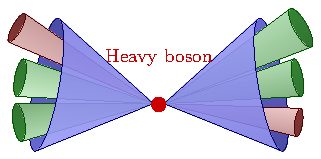
\includegraphics[width=2.5 in]{Images/Chap5/DecayingHeavyBoson.pdf}
    \caption{Schematic drawing of a heavy boson decaying into two large-radius jets (blue cones) with substructure, both normal (green cones) and anomalous (red cones).}
    \label{fig:ADJJ/dataset/states/HBdecay}
\end{figure}

%-------------------------------------------------------------------------------
\subsection{Signal processes}\label{sec:ADJJ/dataset/Signal}

Despite the model-agnostic nature of the AD approach, a set of benchmark signal processes has to be chosen to test the sensitivity of the technique.
In this analysis, two main physical processes are considered: Heavy Vector Triplet (Sec. \ref{sec:SM_BSM/BSM/HVT}) and Dark Jets (Sec. \ref{sec:SM_BSM/BSM/DJ}).\\
The Dark sector is probed using a sample of a $Z'$ boson with mass $m_{Z'} = 3.5 \text{ TeV}$, decaying into a pair of dark quarks with a mass $m_{q_D} = 20 \text{ GeV}$ each .\\
HVT, instead, are explored with three different processes.
The first one is the decay of a heavy vector boson $V$, assumed to be the candidate $Y$ boson, into a BSM vector boson $X$ and the SM Higgs boson $H$.
The masses of the $V$ and $X$ bosons are varied in order to explore different kinematic configurations, among $m_V = [2.3 , 3.4 , 5.0 , 6.0 ] \text{ TeV}$ and $m_X = [100 , 200, 2500, 400] \text{ GeV}$ respectively.
The mass of the Higgs boson, instead, is fixed to its SM value of $m_H = 125 \text{ GeV}$.\\
The second HVT process considered is the decay of a heavy vector boson $V$, into a pair of SM $W$ bosons.
Once again, the mass of the $V$ boson is varied among $m_V = [2.0 , 3.0 , 4.0 , 5.0 ] \text{ TeV}$, while the masses of the $W$ bosons are fixed to their SM value of $m_W = 80 \text{ GeV}$.\\
In conclusion, the third process studied is the decay of a heavy $W'$ boson into a $W$ and a $Z$ BSM bosons, with single masses at $m_{W'} = 3.0 \text{ TeV}$, $m_W = 200 \text{ GeV}$ and $m_Z = 400 \text{ GeV}$.\\
In all the three cases, bosons are assumed to decay into quarks, forming jets in the final state.\\
The complete list of signal processes considered in the analysis, together with their corresponding masses and theoretical cross-sections assumed, is reported in Tab. \ref{tab:sec:ADJJ/dataset/Signal}.
The theoretical cross-sections are derived from the ATLAS internal database for $MC23d$ campaign.

\begin{table}[htbp]
\raggedright
\begin{tabular}{|c|c||c||c|}
\hline
\rowcolor{lightgray}
\textbf{Signal Name} & \textbf{Process} & \textbf{Masses [GeV]} & \shortstack{\textbf{Theoretical}\\\textbf{cross-section [pb]}} \\
\hline\hline 

 VcXH & $V \to XH$ & $m_V = 2300$, $m_X = 100$ & $4.7435 \cdot 10^{-1}$ \\
 VcXH & $V \to XH$ & $m_V = 3400$, $m_X = 200$ & $4.1550 \cdot 10^{-2}$ \\
 VcXH & $V \to XH$ & $m_V = 5000$, $m_X = 2500$ & $1.6359 \cdot 10^{-3}$ \\
 VcXH & $V \to XH$ & $m_V = 6000$, $m_X = 400$ & $2.1811 \cdot 10^{-4}$ \\
\hline

 VzWW & $V \to WW$ & $m_V = 2000$ & $3.8476 \cdot 10^{-3}$ \\
 VzWW & $V \to WW$ & $m_V = 3000$ & $3.5969 \cdot 10^{-4}$ \\
 VzWW & $V \to WW$ & $m_V = 4000$ & $4.5256 \cdot 10^{-5}$ \\
 VzWW & $V \to WW$ & $m_V = 5000$ & $6.2648 \cdot 10^{-6}$ \\
\hline
 
 Wprime & $W' \to WZ$ & $m_{W'} = 3000$, $m_W = 200$, $m_Z = 400$ & $9.6982 \cdot 10^{-16}$ \\
\hline
 
 DarkJet & $Z' \to q_D \bar{q}_D$ & $m_{Z'} = 3500$, $m_{q_D} = 20$, $m_{q_D} = 20$ & $1.05853 \cdot 10^{-9}$ \\
\hline
 
\end{tabular}
\caption{Signal processes considered in the analysis, with their corresponding masses and theoretical cross-sections.}
\label{tab:sec:ADJJ/dataset/Signal}
\end{table}

%-------------------------------------------------------------------------------
\subsection{Background processes}\label{sec:ADJJ/dataset/BKG}


\begin{figure}[ht!]
    \centering
    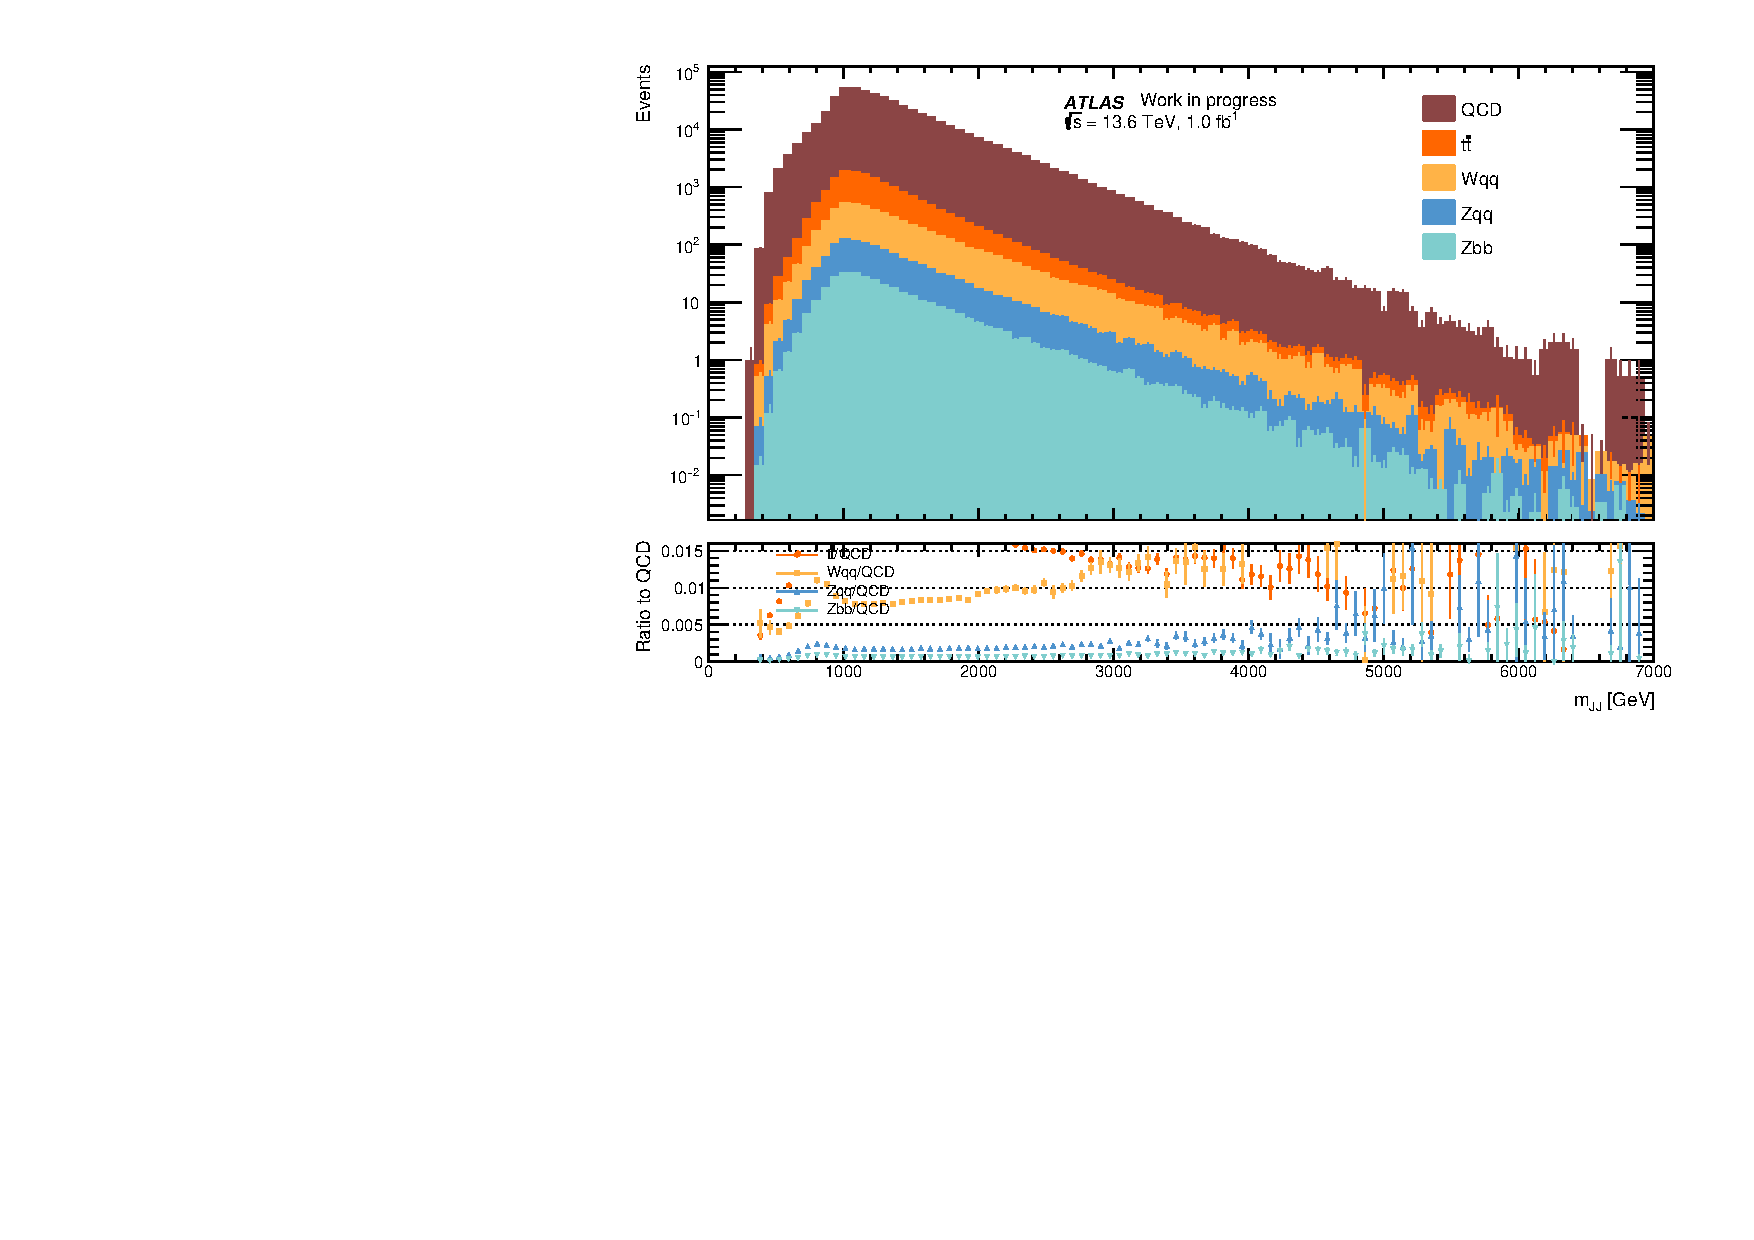
\includegraphics[width=4.5 in]{Images/Chap5/DataPlots/BKG_stack.pdf}
    \caption{Stacked distribution of the di-jet invariant mass $m_{JJ}$ for the dominant background processes considered in the analysis.}
    \label{fig:ADJJ/dataset/BKG/BKGstack}
\end{figure}

%-------------------------------------------------------------------------------
%-------------------------------------------------------------------------------
\section{Machine Learning }\label{sec:ADJJ/GNN}



%%%%%%%%%%%%%%%%%%%%%%%%%%%%%%%%%
%%%%%%%%%%%%%%%%%%%%%%%%%%%%%%%%%

\section{Graph Neural Networks}
\label{sec:gnn}

Particle physics events inherently feature variable numbers of reconstructed objects—such as tracks, topological clusters, or jet constituents—interacting within complex geometrical spaces. Graph Neural Networks (GNNs) exploit this structure by representing collision events as sparse directed graphs $G = (V, E)$, where nodes $v_i \in V$ correspond to individual particles or sub-detectors, and edges $e_{ij} \in E$ parameterize relational features or spatial separations $\Delta R = \sqrt{(\Delta\eta)^2 + (\Delta\phi)^2}$.

Node feature vectors $h_i^{(0)}$ encode basic spatial and kinematic observables, including transverse momentum $p_T$, pseudorapidity $\eta$, azimuthal angle $\phi$, and impact parameters. Graph neural architectures process relational topology through Message Passing Neural Network (MPNN) frameworks. At execution step $t$, node representations are updated iteratively using localized neighborhood information:
\begin{equation}
    m_i^{(t+1)} = \sum_{j \in \mathcal{N}(i)} \mathcal{M}_{\theta} \left( h_i^{(t)}, h_j^{(t)}, e_{ij} \right)
\end{equation}
\begin{equation}
    h_i^{(t+1)} = \mathcal{U}_{\phi} \left( h_i^{(t)}, m_i^{(t+1)} \right)
\end{equation}
where $\mathcal{N}(i)$ defines the set of immediate spatial neighbors of node $i$, $\mathcal{M}_{\theta}$ represents a parameterized message function, and $\mathcal{U}_{\phi}$ constitutes a node-state update function.

Permutation invariance across input node orderings is enforced via global pooling operations:
\begin{equation}
    h_G = \bigoplus_{v_i \in V} h_i^{(T)}
\end{equation}
where $\bigoplus$ represents a symmetric aggregation operator such as a element-wise summation, mean, or attention-weighted sum. In the context of large-radius jet substructure analyses within ATLAS, GNN architectures capture complex inter-particle correlations, color-flow dynamics, and energy distributions without relying on manually engineered substructure variables such as $N$-subjettiness $\tau_N$ or energy correlation functions $D_2$.

\section{Anomaly Detection Implementation with Deep Learning}
\label{sec:ad_implementation}

Deep-learning-based Anomaly Detection in High Energy Physics is operationalized through distinct architectural formulations:

\textbf{Self-Supervised Reconstruction Architectures:} Autoencoders (AEs) compress input vectors $x \in \mathbb{R}^d$ into a lower-dimensional latent representation $z \in \mathbb{R}^k$ ($k \ll d$) via an encoding network $f_\theta(x)$, subsequently reconstructing the input via a decoding network $g_\phi(z)$. Trained exclusively on dominant SM background events using loss metrics such as Mean Squared Error:
\begin{equation}
    \mathcal{L}_{\text{MSE}} = \| x - g_\phi(f_\theta(x)) \|^2
\end{equation}
the AE optimizes loss metrics for standard topologies. When evaluated on BSM topologies absent from training ensembles, the AE fails to accurately reconstruct the anomalous features, yielding significantly elevated reconstruction errors. These errors directly construct a continuous Anomaly Score (AS). Variational Autoencoders (VAEs) regularize this latent space by enforcing a standard Gaussian prior distribution $p(z) \sim \mathcal{N}(0, I)$ through a Kullback-Leibler divergence term $\mathcal{D}_{\text{KL}}$, balancing latent space continuity against reconstruction fidelity.

\textbf{Weakly-Supervised Overdensity Estimation:} The Classification Without Labels (CWoLa) paradigm isolates overdensities in resonant spectra by establishing mixed signal-plus-background datasets. Defining a Signal Region (SR) in a invariant mass continuum $m_{JJ}$ alongside adjacent Control Sidebands (SB), a classifier is trained directly on unlabeled experimental data to distinguish SR events from SB events. By the Neyman-Pearson Lemma, a classifier trained on mixed ensembles with differing signal proportions converges monotonically to the optimal Likelihood Ratio:
\begin{equation}
    R(x) = \frac{p_{\text{data}}(x | m \in \text{SR})}{p_{\text{bg}}(x | m \in \text{SR})}
\end{equation}

Advanced weakly-supervised density estimators, such as CATHODE, CURTAINS, and ANODE, employ conditional normalizing flows or optimal transport algorithms to model sideband background dynamics, interpolating background probability densities directly into the SR to eliminate feature correlations and artificial mass sculpting.

In the ATLAS ADJJ (Anomaly Detection in Dijet final states) analysis, GNN architectures are interfaced directly with model-independent search frameworks. Unsupervised GNN autoencoders process the constituent point-clouds of large-radius anti-$k_t$ ($R=1.0$) jets, outputting an Anomaly Score for every event. Selecting thresholds on the AS distribution defines specific Working Points (WPs), achieving background rejection factors spanning orders of magnitude. 

Model-independent signal searches are subsequently executed by scanning the di-jet invariant mass $m_{JJ}$ spectrum across defined AS WPs. Smooth parametric functions model the suppressed SM background background continuum, while potential anomalous signals are evaluated using flexible resonance fits, such as Double-Sided Crystal Ball functions. Binned maximum likelihood fits combined with the $\text{CL}_s$ statistical method derive 95\% Confidence Level upper limits on production cross-sections, providing a sensitivity bridge between deep graph representations and model-agnostic BSM discoveries at CERN.



%%%%%%%%%%%%%%%%%%%%%%%%%%%%%%%%%%
\section{Overview of Anomaly Detection}
\label{sec:ad_overview}

Anomaly Detection encompasses algorithms that identify data instances deviating significantly from nominal distributions \cite{belis2023machine, tinari2024}. 
In standard industrial contexts, anomalies manifest as out-of-sample or off-manifold events, such as fraudulent transactions or equipment failures \cite{kasieczka2021lhc, tinari2024}. 
In High Energy Physics (HEP), single events rarely provide statistical evidence of new phenomena; BSM signals typically manifest as subtle over-densities in phase space \cite{belis2023machine, kasieczka2021lhc}.

Within particle physics, ML-based AD strategies operate across different levels of supervision \cite{belis2023machine, tinari2024}. 
Weakly supervised methods, such as Classification Without Labels (CWoLa) and CATHODE, estimate localized over-densities by comparing signal-enriched regions against adjacent sidebands \cite{belis2023machine, tinari2024}. 
Conversely, fully unsupervised methods operate solely on background processes or unlabeled experimental data \cite{belis2023machine, tinari2024}. 
These algorithms isolate rare topology features in kinematic distributions, providing an unbiased tool for model-agnostic BSM searches \cite{belis2023machine, davide_proc}.


\section{Graph Neural Networks}\label{sec:gnn}
Standard feedforward architectures struggle to process variable-size physical objects without imposing artificial ordering \cite{dav_ad_proc, Russo_thesis}. Hadronic jets, composed of varying counts of collimated sub-particles, naturally map to graph structures $G = (V, E)$, where $V$ denotes constituent nodes and $E$ represents interaction edges \cite{kasieczka2021lhc, davide_proc}. Node features contain kinematic variables $\mathbf{x}_i = (p_T, \eta, \phi)$, while edge features capture pairwise angular separations $\Delta R = \sqrt{(\Delta \eta)^2 + (\Delta \phi)^2}$ \cite{kasieczka2021lhc, davide_proc}.Graph Neural Networks (GNNs) preserve permutation invariance while executing local message passing \cite{kasieczka2021lhc, davide_proc}. The representation $\mathbf{h}_i^{(l)}$ of node $i$ at layer $l$ updates according to aggregated messages from its spatial neighborhood $\mathcal{N}(i)$ \cite{davide_proc}:\begin{equation}\mathbf{m}_{ij}^{(l)} = \phi_e \left( \mathbf{h}_i^{(l-1)}, \mathbf{h}j^{(l-1)}, \mathbf{e}{ij} \right)\end{equation}\begin{equation}\mathbf{h}i^{(l)} = \phi_v \left( \mathbf{h}i^{(l-1)}, \bigoplus{j \in \mathcal{N}(i)} \mathbf{m}{ij}^{(l)} \right)\end{equation}where $\phi_e$ and $\phi_v$ denote neural operations, $\mathbf{e}_{ij}$ is the edge feature, and $\bigoplus$ represents a permutation-invariant aggregation operator such as sum, mean, or max \cite{kasieczka2021lhc, davide_proc}. Graph-level outputs obtain global representations via permutation-invariant pooling functions across all nodes \cite{davide_proc}.

\section{Anomaly Detection Implementation via Deep Architectures}\label{sec:ad_implementation}
Unsupervised AD implementation utilizing DNNs and GNNs relies on latent representation learning \cite{belis2023machine, tinari2024}. Autoencoders (AEs) compress input graph representations $\mathbf{x}$ into a lower-dimensional bottleneck $\mathbf{z} = f_{\text{enc}}(\mathbf{x})$ before generating a reconstructed output $\hat{\mathbf{x}} = f_{\text{dec}}(\mathbf{z})$ \cite{belis2023machine, tinari2024}. When trained exclusively on dominant Standard Model background events, the network learns lossy compression tailored to nominal physics patterns \cite{belis2023machine, davide_proc}.Events containing BSM physics produce higher reconstruction errors due to unlearned substructure features \cite{belis2023machine, tinari2024}. An Anomaly Score ($AS$) is defined using the Mean Squared Error (MSE) metric \cite{belis2023machine, dav_ad_proc}:\begin{equation}AS = \frac{1}{N} \sum_{i=1}^{N} \left| \mathbf{x}_i - \hat{\mathbf{x}}_i \right|^2\end{equation}In ATLAS model-independent searches, cuts applied to the calculated $AS$ distribution isolate BSM candidates \cite{belis2023machine, davide_proc}. By filtering out high-probability background interactions, these architectures define signal-enriched regions directly from data, enabling model-agnostic resonance searches \cite{belis2023machine, tinari2024}.

% #################################################à
\section{CURCH}\label{sec:WhatisAD}


%%%%%%%%%%%%%%%%%%


%%%%%%%%%%%%%%%%%%%%%%
\section{How is it implemented?}\label{sec:ADimplementation}
The process of training a  DL model is divided into three main phases: training, validation and test loop. They are defined "loop" because in each of them a different section of the dataset is used and the code loops over it.\\
The most important stage is the training loop: in our case the chosen DL model is trained to reconstruct arrays containing information about particle jets, using only data with normal behaviour (background events) \cite{DLforAD}. In this phase, parameters of the model are adjusted in order to best fit to data. By doing so, DL model is able to recognise very well normal data and their structure. Our hope is that, once it faces an anomaly (signal event), it is able to identify it due to its difference from what it knows. The second step is the validation loop, where a valuation of the performance of the model is elaborated using the validation set. The valuation and the search for the best weights of the model are executed computing distance between output and input over training and validation set. When this distance is minimum within the validation loop, we save the model's weights.\\
The trained and tuned model is then tested, using a dataset containing unseen data, the test set, where there are both background and signal events. The purpose of this phase is to validate results previously obtained and get a preview of what will happen once the model will be running with completely new data. The task is completed computing the Anomaly Score (AS). In this thesis, we implement it as a distance between input and output, with different dimension: instead of calculating it over a batch of data, we do so for each event. In this way we are able to plot a reconstruction probability graph: we expect that the distributions of AS from background and signal events are different, because signal data contains anomalies which our model does not know. By means of these distributions we can identify a threshold of separation between them. For any event we pass to our trained model, we compute AS: if it higher (lower) than the chosen threshold, we are looking at a background (signal) event. Since AD is distinguishing signal events from background, we are basically executing a classification task with two classes. Implementation of Anomaly Detection is discussed more in depth in chapters \ref{chap:Model} and \ref{chap:Results}.

% \begin{figure}[h!]
%     \centering
%     \includegraphics[width=3 in]{Images/Cap3/ADtestloop.png}
%     \caption{Test loop of Anomaly Detection. Figure from Ref. \cite{DLforAD}}
%     \label{fig:RECOprob}
% \end{figure}

